\chapter{Implementation Concept}

The most promising vector tiles specification was proposed by Mapbox.
\marginpar{The Mapbox Vector Tile Specification is compared with other vector tile formats in chapter \ref{vector-tile-formats}}
They provide many open source tools to manage vector tiles. We tried not to implement tools which already exists and instead use as many existing tools as possible. Because of this our implementation consists mostly of docker containers which do a specific task.

\section{Vector Tile Rendering}

\paragraph{Data Style} The data style is a description of the different feature sets such as landuse, water or roads together with its sql query. The sql query defines which data needs to be fetched on which zoomlevel.

The figure below shows the high level workflow of the vector tile rendering process. On the left side are the data sources, which get imported into a Postgis database. The import tools map the data sources to a database table and create indices for fast querying during the rendering process.
The vector tile renderer takes the data style as input and queries the PostGIS database for the required feature sets necessary for one vector tile.


\begin{figure}[h]
  \centering
  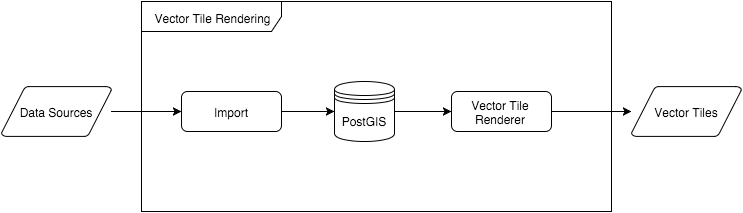
\includegraphics[width=1\textwidth]{images/vector_tile_rendering.png}
  \caption{Vector Tile Rendering Process}
\end{figure}

\section{Tile Server}

\paragraph{Visual Style} The visual style defines how a feature set such as landuse actually looks. In the case of landuse on could define the texture, color of the border and area.

\subsection{Raster Tile Server}

The raster tile server makes it possible to view the vector tiles. The output of the vector tile rendering process is just the raw vector data. To view the vector tiles we need a visual style, which defines how the defined feature sets in the data source should look like. The visual style defines for example that the feature set landuse should have a green color or that water should be blue. In the figure below we can see on the left side our vector tiles (mbtiles) and the visual style (TM2 Style). Tessera takes these two items and delivers them to mapnik which generates raster tiles. Tessera automatically starts a webserver and serves the generated raster tiles.

\begin{figure}[h]

  \centering
  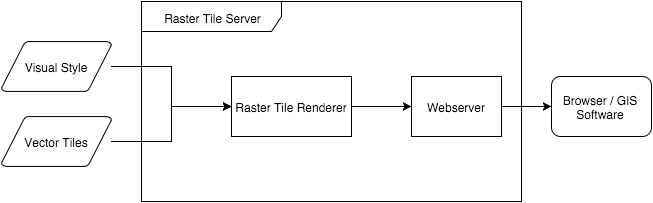
\includegraphics[width=1\textwidth]{images/raster_tile_server.png}
  \caption{Raster tile server}
\end{figure}

\subsection{Vector Tile Server}

\begin{figure}[h]

  \centering
  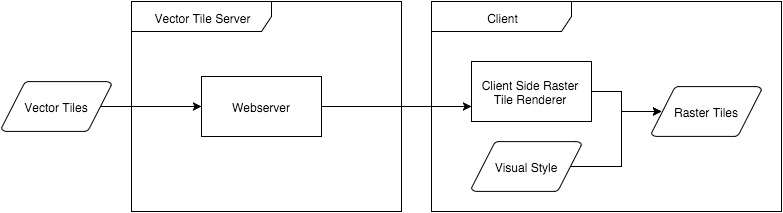
\includegraphics[width=1\textwidth]{images/vector_tile_server.png}
  \caption{Vector tile server}
\end{figure}



\newpage